%
%
%
% - - - - - Prototyp - - - - - - - - 
%
%
%
\chapter{Prototyp zur Unterstützung in der Sterilgutversorgung}
\label{ch:Prototyp}
Implementiert wurde ein Prototyp für die \emph{Realwear hmt-1}. Der Prototyp einer multimedialen Smartglass- Anwendung ermöglicht es, Videos auf einer hmt-1 abzuspielen sowie aufzuzeichnen und eine Slideshow von Bildern abzuspielen. 
\insertMore{Prototyp}
%
%
%
% - - - - - Verwendete Technologien - - - - - - - - 
%
%
%
\section{Verwendete Technologien}
\label{sec:Verwendete_Technologien}
\insertMore{Verwendete Technologien}
% 3 Seiten
%
%
%
% - - - - - Implementation - - - - - - - - 
%
%
%
\section{Implementation}
\label{sec:Implementation}
%
%
%
% - - - - - User-Interface - - - - - - - - 
%
%
%
\subsection{User-Interface}
Die Android-Anwendung wurde nach dem in Abbildung \ref{fig:Storyboard_des_Prototypen} gezeigten Storyboard erstellt. Die Anwendung beginnt in einem Hauptmenü, welches ermöglicht, per Sprachbefehl einen von drei Buttons auszuwählen. Mit dem ersten Button wird der Nutzer zur Slideshow-Seite weitergeleitet. Beim zweiten Button wird auf die Videoanzeige und beim dritten Button auf die Video-Aufzeichnen Funktion weitergeleitet. Mittels eines \enquote{Schritt zurück}- Befehls der Smartglass wird der Androidtypische Zurückbutton betätigt.
%
\begin{figure}[htbp]
    \centering
    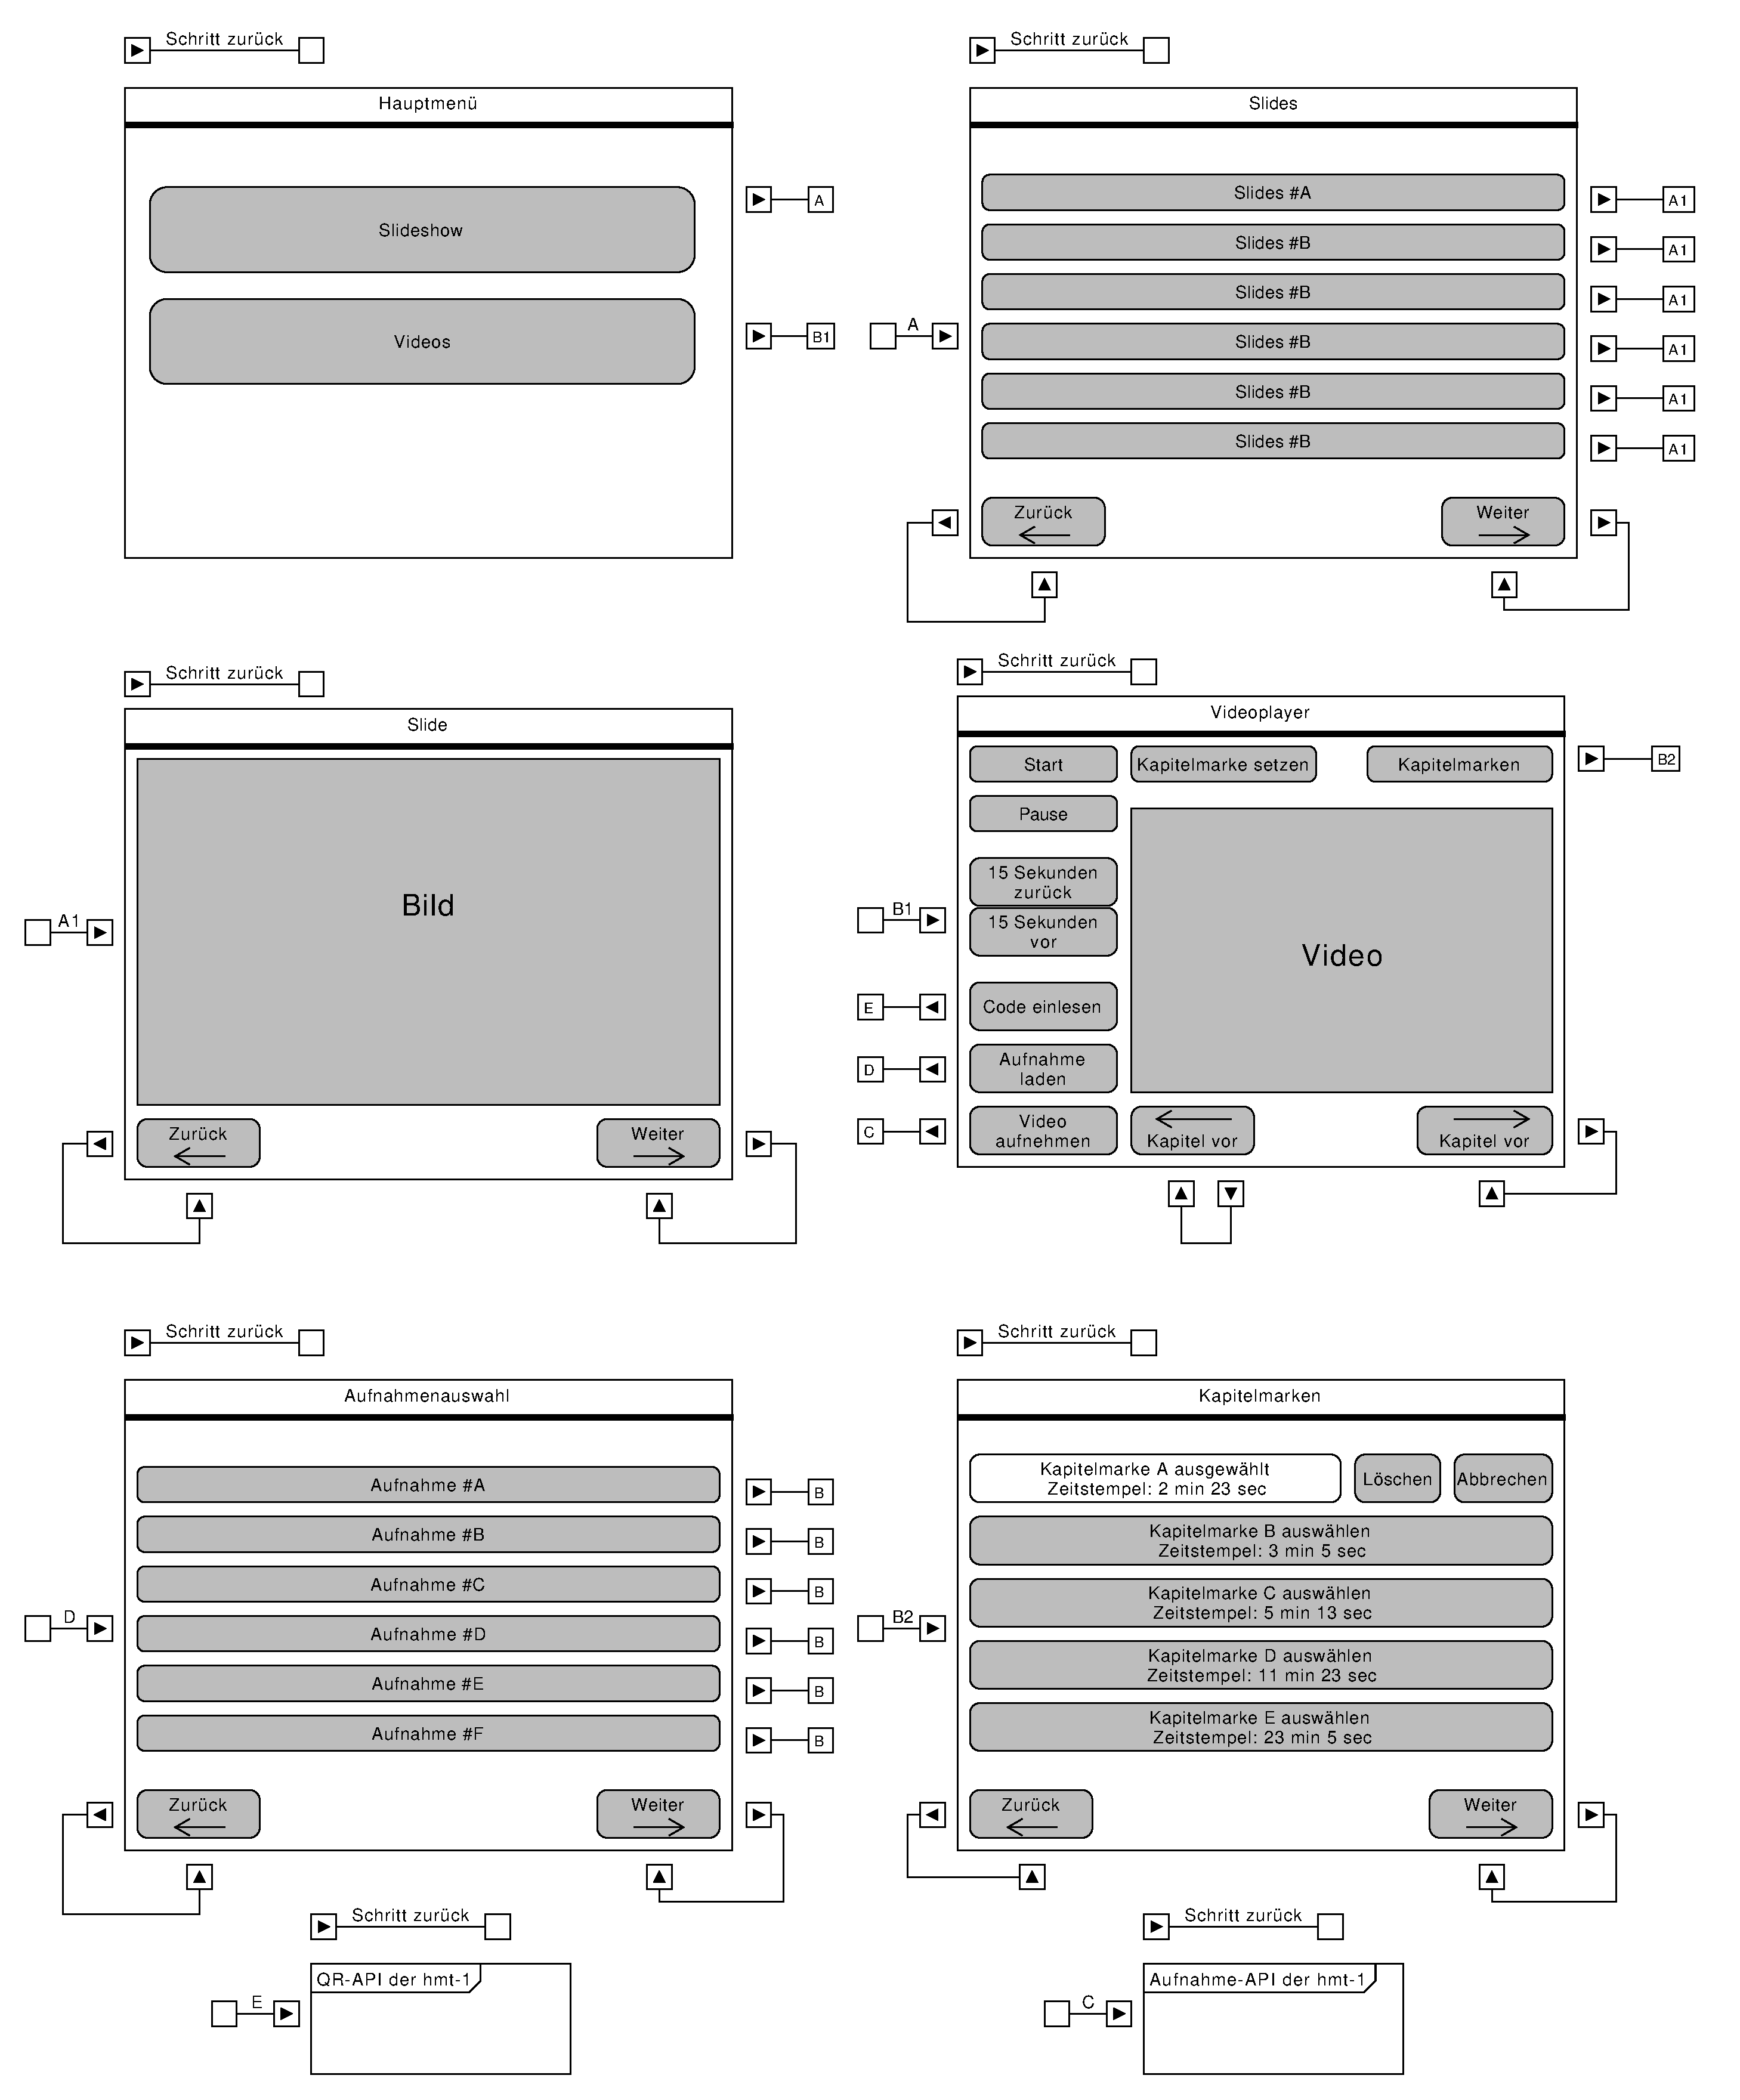
\includegraphics[width=1\textwidth]{data/bilder/UI-Storyboard.pdf}
    \caption{Storyboard des Prototypen}
    \label{fig:Storyboard_des_Prototypen}
\end{figure}

Die Slideshow besteht aus zwei Ansichtstypen. In der ersten Ansicht, welche über das Hauptmenü erreichbar ist, wird eine Liste von Buttons angezeigt, über die einzelne Slides ausgewählt werden können. Am unteren Rand des Fensters ist ein \enquote{Weiter}- Button, welcher die Liste der Buttons aktualisiert, um weitere Slides zur Auswahl zu stellen. Dies ist notwendig, da bei der \emph{hmt-1} scrollen durch eine Liste nicht möglich ist.

Wird eine Bilderliste ausgewählt, so wird auf eine Unterseite verlinkt. Diese besteht aus einem \emph{Image-View} sowie zwei Buttons: \enquote{vorwärts} und \enquote{zurück}. Im Bild wird das aktuelle Bild der Bilderliste angezeigt. Mit \enquote{weiter} wird das nächste, mit \enquote{zurück} das vorherige Bild angezeigt.

Aus dem Hauptmenü kann zudem die \emph{Videoplayer}- Ansicht geöffnet werden. Diese Ansicht besteht aus zwei Bereichen. Links ist eine Sammlung von insgesamt 7 Buttons zum starten und stoppen, vor- und zurückspulen des Videos um 15 Sekunden, Einlesen eines QR-Codes und einlesen des Videolinks in den Videoplayer. Zusätzlich sind noch zwei Buttons zum Aufnehmen eines Videos und zum Laden einer Aufnahme in den Player. Rechts ist ein Videofenster angebracht, in dem die Videos angezeigt werden.

Wählt ein Nutzer den \enquote{Aufnahmen auswählen}- Button, so wird ein Fenster geöffnet, welches ähnlich dem \enquote{Slide}-Fenster aufgebaut ist. Auch hier ist eine Liste sowie ein Weiter-Button, welcher genauso funktioniert wie in der \endquote{Slide}- View. Wird eine Aufnahme ausgewählt, wird diese in den Videoplayer geladen.

Einlesen des QR-Codes sowie die Aufnahme des Videos werden mithilfe der API der \emph{hmt-1} realisiert und das jeweilige Ergebnis an die aufrufende View übergeben.

\insertMore{Implementation}
% 3 Seiten